\documentclass{standalone}
\usepackage{tikz}
\usetikzlibrary{patterns, positioning}

\begin{document}
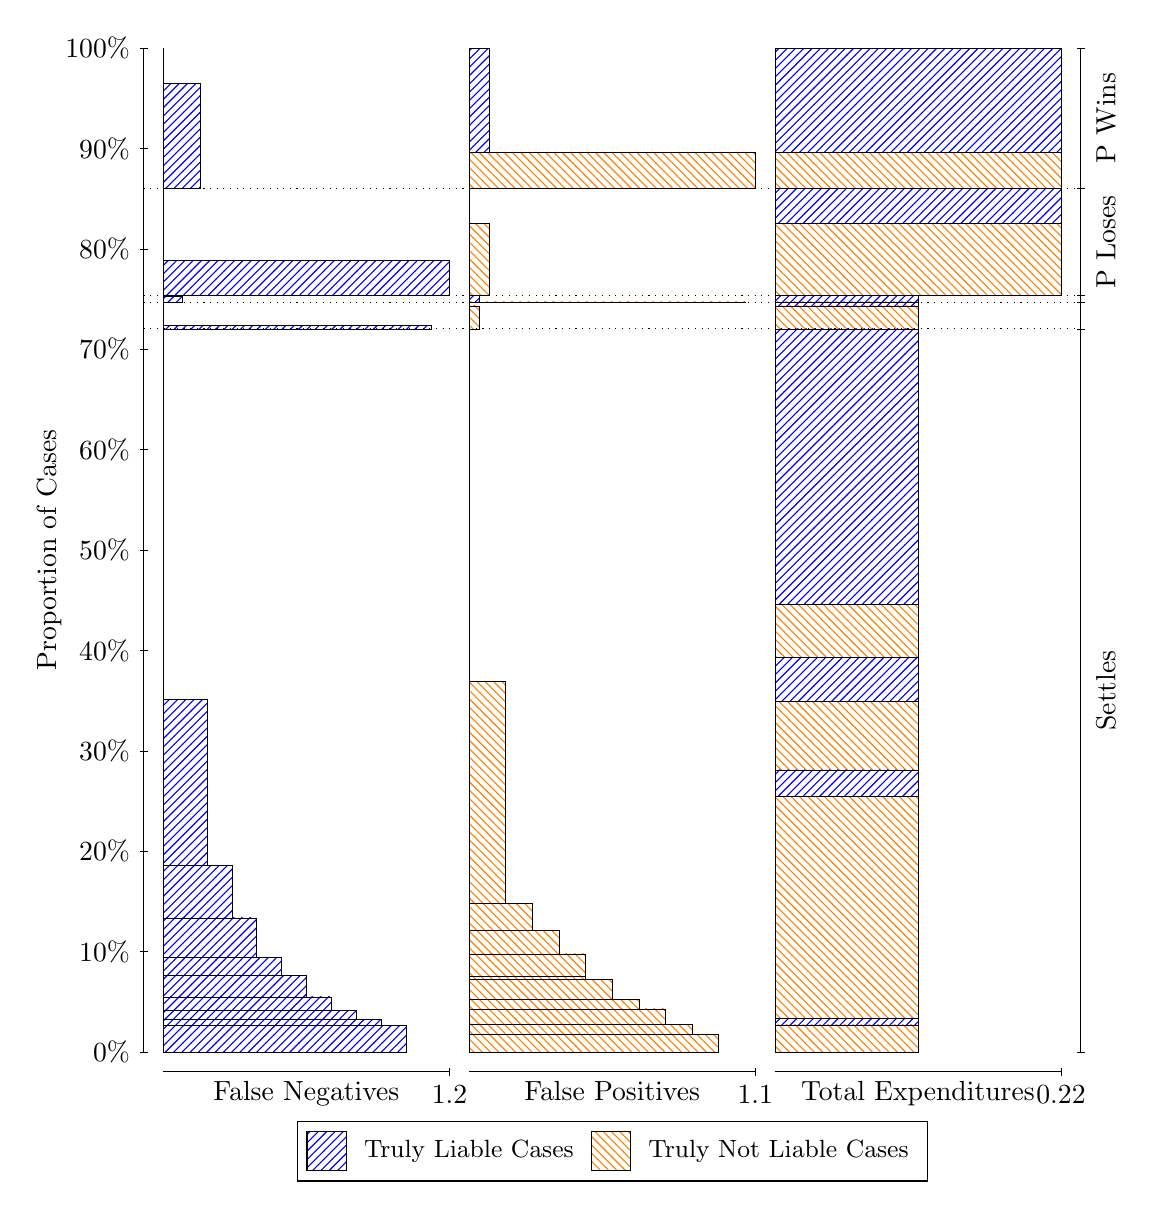
\begin{tikzpicture}
\draw[black, very thin] (1.5,1.75) -- (1.5,14.5);
\node[rotate=90, anchor=center] at (0.3, 8.125) {Proportion of Cases};
\draw[black, very thin] (1.45,1.75) -- (1.55,1.75);
\node[anchor=east] at (1.45, 1.75) {0\%};
\draw[black, very thin] (1.45,3.025) -- (1.55,3.025);
\node[anchor=east] at (1.45, 3.025) {10\%};
\draw[black, very thin] (1.45,4.3) -- (1.55,4.3);
\node[anchor=east] at (1.45, 4.3) {20\%};
\draw[black, very thin] (1.45,5.575) -- (1.55,5.575);
\node[anchor=east] at (1.45, 5.575) {30\%};
\draw[black, very thin] (1.45,6.85) -- (1.55,6.85);
\node[anchor=east] at (1.45, 6.85) {40\%};
\draw[black, very thin] (1.45,8.125) -- (1.55,8.125);
\node[anchor=east] at (1.45, 8.125) {50\%};
\draw[black, very thin] (1.45,9.4) -- (1.55,9.4);
\node[anchor=east] at (1.45, 9.4) {60\%};
\draw[black, very thin] (1.45,10.675) -- (1.55,10.675);
\node[anchor=east] at (1.45, 10.675) {70\%};
\draw[black, very thin] (1.45,11.95) -- (1.55,11.95);
\node[anchor=east] at (1.45, 11.95) {80\%};
\draw[black, very thin] (1.45,13.225) -- (1.55,13.225);
\node[anchor=east] at (1.45, 13.225) {90\%};
\draw[black, very thin] (1.45,14.5) -- (1.55,14.5);
\node[anchor=east] at (1.45, 14.5) {100\%};

\draw[black, very thin] (13.4,1.75) -- (13.4,14.5);
\draw[black, very thin] (13.35,1.75) -- (13.45,1.75);
\node[anchor=west] at (13.35, 1.75) {};
\draw[black, very thin] (13.35,10.934) -- (13.45,10.934);
\node[anchor=west] at (13.35, 10.934) {};
\draw[black, very thin] (13.35,11.269) -- (13.45,11.269);
\node[anchor=west] at (13.35, 11.269) {};
\draw[black, very thin] (13.35,11.355) -- (13.45,11.355);
\node[anchor=west] at (13.35, 11.355) {};
\draw[black, very thin] (13.35,12.721) -- (13.45,12.721);
\node[anchor=west] at (13.35, 12.721) {};
\draw[black, very thin] (13.35,14.5) -- (13.45,14.5);
\node[anchor=west] at (13.35, 14.5) {};

\draw[black, very thin, pattern color=blue, pattern=north east lines] (1.75,1.75) rectangle (4.8304,2.0862);
\draw[black, very thin, pattern color=blue, pattern=north east lines] (1.75,2.0862) rectangle (4.5145,2.1654);
\draw[black, very thin, pattern color=blue, pattern=north east lines] (1.75,2.1654) rectangle (4.1986,2.2792);
\draw[black, very thin, pattern color=blue, pattern=north east lines] (1.75,2.2792) rectangle (3.8826,2.4485);
\draw[black, very thin, pattern color=blue, pattern=north east lines] (1.75,2.4485) rectangle (3.5667,2.7217);
\draw[black, very thin, pattern color=blue, pattern=north east lines] (1.75,2.7217) rectangle (3.2507,2.9522);
\draw[black, very thin, pattern color=blue, pattern=north east lines] (1.75,2.9522) rectangle (2.9348,3.454);
\draw[black, very thin, pattern color=blue, pattern=north east lines] (1.75,3.454) rectangle (2.6188,4.1189);
\draw[black, very thin, pattern color=blue, pattern=north east lines] (1.75,4.1189) rectangle (2.3029,6.2252);
\draw[black, very thin, pattern color=orange, pattern=north west lines] (1.75,6.2252) rectangle (1.75,10.934);
\draw[black, very thin, pattern color=blue, pattern=north east lines] (1.75,10.934) rectangle (5.1464,10.978);
\draw[black, very thin, pattern color=orange, pattern=north west lines] (1.75,10.978) rectangle (1.75,11.269);
\draw[black, very thin, pattern color=blue, pattern=north east lines] (1.75,11.269) rectangle (1.987,11.347);
\draw[black, very thin, pattern color=orange, pattern=north west lines] (1.75,11.347) rectangle (1.75,11.355);
\draw[black, very thin, pattern color=blue, pattern=north east lines] (1.75,11.355) rectangle (5.3833,11.802);
\draw[black, very thin, pattern color=orange, pattern=north west lines] (1.75,11.802) rectangle (1.75,12.721);
\draw[black, very thin, pattern color=blue, pattern=north east lines] (1.75,12.721) rectangle (2.2239,14.051);
\draw[black, very thin, pattern color=orange, pattern=north west lines] (1.75,14.051) rectangle (1.75,14.5);
\draw[black, very thin, pattern color=orange, pattern=north west lines] (5.6333,1.75) rectangle (8.8019,1.9743);
\draw[black, very thin, pattern color=orange, pattern=north west lines] (5.6333,1.9743) rectangle (8.464,2.1042);
\draw[black, very thin, pattern color=orange, pattern=north west lines] (5.6333,2.1042) rectangle (8.126,2.2974);
\draw[black, very thin, pattern color=orange, pattern=north west lines] (5.6333,2.2974) rectangle (7.788,2.4199);
\draw[black, very thin, pattern color=orange, pattern=north west lines] (5.6333,2.4199) rectangle (7.45,2.6701);
\draw[black, very thin, pattern color=orange, pattern=north west lines] (5.6333,2.6701) rectangle (7.112,2.7079);
\draw[black, very thin, pattern color=orange, pattern=north west lines] (5.6333,2.7079) rectangle (7.112,2.9961);
\draw[black, very thin, pattern color=orange, pattern=north west lines] (5.6333,2.9961) rectangle (6.774,3.2929);
\draw[black, very thin, pattern color=orange, pattern=north west lines] (5.6333,3.2929) rectangle (6.436,3.6375);
\draw[black, very thin, pattern color=orange, pattern=north west lines] (5.6333,3.6375) rectangle (6.0981,6.4588);
\draw[black, very thin, pattern color=blue, pattern=north east lines] (5.6333,6.4588) rectangle (5.6333,10.934);
\draw[black, very thin, pattern color=orange, pattern=north west lines] (5.6333,10.934) rectangle (5.7601,11.225);
\draw[black, very thin, pattern color=blue, pattern=north east lines] (5.6333,11.225) rectangle (5.6333,11.269);
\draw[black, very thin, pattern color=orange, pattern=north west lines] (5.6333,11.269) rectangle (9.1399,11.277);
\draw[black, very thin, pattern color=blue, pattern=north east lines] (5.6333,11.277) rectangle (5.7601,11.355);
\draw[black, very thin, pattern color=orange, pattern=north west lines] (5.6333,11.355) rectangle (5.8868,12.273);
\draw[black, very thin, pattern color=blue, pattern=north east lines] (5.6333,12.273) rectangle (5.6333,12.721);
\draw[black, very thin, pattern color=orange, pattern=north west lines] (5.6333,12.721) rectangle (9.2667,13.17);
\draw[black, very thin, pattern color=blue, pattern=north east lines] (5.6333,13.17) rectangle (5.8868,14.5);
\draw[black, very thin, pattern color=orange, pattern=north west lines] (9.5167,1.75) rectangle (11.333,2.0946);
\draw[black, very thin, pattern color=blue, pattern=north east lines] (9.5167,2.0946) rectangle (11.333,2.1737);
\draw[black, very thin, pattern color=orange, pattern=north west lines] (9.5167,2.1737) rectangle (11.333,4.995);
\draw[black, very thin, pattern color=blue, pattern=north east lines] (9.5167,4.995) rectangle (11.333,5.3312);
\draw[black, very thin, pattern color=orange, pattern=north west lines] (9.5167,5.3312) rectangle (11.333,6.2043);
\draw[black, very thin, pattern color=blue, pattern=north east lines] (9.5167,6.2043) rectangle (11.333,6.7607);
\draw[black, very thin, pattern color=orange, pattern=north west lines] (9.5167,6.7607) rectangle (11.333,7.4305);
\draw[black, very thin, pattern color=blue, pattern=north east lines] (9.5167,7.4305) rectangle (11.333,10.934);
\draw[black, very thin, pattern color=orange, pattern=north west lines] (9.5167,10.934) rectangle (11.333,11.225);
\draw[black, very thin, pattern color=blue, pattern=north east lines] (9.5167,11.225) rectangle (11.333,11.269);
\draw[black, very thin, pattern color=orange, pattern=north west lines] (9.5167,11.269) rectangle (11.333,11.277);
\draw[black, very thin, pattern color=blue, pattern=north east lines] (9.5167,11.277) rectangle (11.333,11.355);
\draw[black, very thin, pattern color=orange, pattern=north west lines] (9.5167,11.355) rectangle (13.15,12.273);
\draw[black, very thin, pattern color=blue, pattern=north east lines] (9.5167,12.273) rectangle (13.15,12.721);
\draw[black, very thin, pattern color=orange, pattern=north west lines] (9.5167,12.721) rectangle (13.15,13.17);
\draw[black, very thin, pattern color=blue, pattern=north east lines] (9.5167,13.17) rectangle (13.15,14.5);
\draw[black, dotted] (1.5,10.934) -- (13.4,10.934);
\draw[black, dotted] (1.5,11.269) -- (13.4,11.269);
\draw[black, dotted] (1.5,11.355) -- (13.4,11.355);
\draw[black, dotted] (1.5,12.721) -- (13.4,12.721);
\draw[black, very thin] (1.75,1.5) -- (5.3833,1.5);
\node[anchor=north] at (3.5667, 1.5) {False Negatives};
\draw[black, very thin] (5.3833,1.45) -- (5.3833,1.55);
\node[anchor=north] at (5.3833, 1.45) {1.2};

\draw[black, very thin] (5.6333,1.5) -- (9.2667,1.5);
\node[anchor=north] at (7.45, 1.5) {False Positives};
\draw[black, very thin] (9.2667,1.45) -- (9.2667,1.55);
\node[anchor=north] at (9.2667, 1.45) {1.1};

\draw[black, very thin] (9.5167,1.5) -- (13.15,1.5);
\node[anchor=north] at (11.333, 1.5) {Total Expenditures};
\draw[black, very thin] (13.15,1.45) -- (13.15,1.55);
\node[anchor=north] at (13.15, 1.45) {0.22};

\node[black, centered, rotate=90] at (13.72, 6.342) {Settles};


\node[black, centered, rotate=90] at (13.72, 12.038) {P Loses};
\node[black, centered, rotate=90] at (13.72, 13.61) {P Wins};

\draw (7.449999999999999,1.5) node[draw=none] (baseCoordinate) {};
\begin{scope}[align=center]
        \matrix[scale=0.5, draw=black, below=0.5cm of baseCoordinate, nodes={draw}, column sep=0.1cm]{
            \node[rectangle, draw, minimum width=0.5cm, minimum height=0.5cm, pattern=north east lines, pattern color=blue] {}; &
            \node[draw=none, font=\small] (B) {Truly Liable Cases}; &
            \node[rectangle, draw, minimum width=0.5cm, minimum height=0.5cm, pattern=north west lines, pattern color=orange] {}; &
            \node[draw=none, font=\small] (B) {Truly Not Liable Cases}; \\
            };
\end{scope}

\end{tikzpicture}
\end{document}